\graphicspath{{chapters/introduction/images/}}
\chapter{Introduction}
\label{chapter:introduction}
Measurements of atmospheric neutrino oscillations, such as those performed in this thesis, require a background of understanding of both atmospheric neutrinos as well as neutrino oscillations. 
A history of neutrinos (Section~\ref{sec:neutrinos}) is used to explain the discovery of the three known flavors of neutrinos as well as the difficulties inherent in the study of these elusive particles.
A discussion of the history of cosmic rays (Section~\ref{sec:cosmic_rays}) explains the source of both the neutrinos (Section~\ref{sec:atmo_nus}) used as signal in this thesis as well as the muons, which form one of the primary backgrounds in the search for atmospheric neutrino oscillations.

The detection of neutrinos is described in two parts.
A discussion of the neutrino interactions (Section~\ref{subsec:interactions}), explains the interactions of neutrinos with matter.
The detection of these interactions through electromagnetic emission is then covered (Section~\ref{sec:detection_methods}).

\section{The History of the Neutrino}
\label{sec:neutrinos}
In 1896, Henri Becquerel discovered radioactivity in uranium \cite{Becquerel}.
Measurements over the following decades showed various types of nuclear decays based on the penetration depth of the ionizing emissions.
Measurements of one type of radioactivity, beta decay, over the following 30 years showed that the production of two observed particles from one parent nucleus: a daughter nucleus and an outgoing electron.
A single body decay of this type produces a known energy spectrum of the daughter nucleus and the electron determined by conservation of energy and momentum, leading to a narrow line emission spectrum.

Contrary to expectations, however, the measurement of energies of the two resulting particles showed wide, continuous spectra \cite{Chadwick}. 
The spectrum provided a major puzzle for physicists due to the contradition with the simple theoretical expectations.
A conundrum for many years, one possible solution was suggested in 1930 by Wolfgang Pauli.
In his letter, Pauli suggested that the conservation of energy and momentum could be saved if "... there could exist in the nuclei electrically neutral particles... which have spin 1/2 and obey the exclusion principle, and additionally different from light quanta in that they do not travel with the velocity of light" \cite{Pauli-Nu}.
The solution to the beta decay puzzle was, then, that this additional "neutron" particle was emitted simultaneously with the observed daughter particles.

Pauli's suggestion provided a way to save the beloved conservation laws in physics, but at the expense of the assumption of a new particle.
The particle, called the "neutron" in Pauli's letter and later renamed the "neutrino" by Fermi, was proposed to be electrically neutral and, therefore, completely undetectable at the time.
Later work \cite{Fermi1934} proposed that the neutrinos interact only via the weak nuclear force, with an interaction strength many orders of magnitude smaller than electromagnetic and strong nuclear forces.
Experimental measurements, sensitive only to electromagnetic forces, therefore could not be used to study neutrinos directly in the same way that other particles may be measured.

It was not until nearly 20 years later, in 1956, that this mystery particle was first detected \cite{Cowan-Reines}. 
In a groundbreaking work, Cowen and Reines performed an experiment at the Savannah River Plant, a nuclear power plant, demonstrating detection of the neutrino.
The experiment, made up of layers of scintillation detectors around polyethelene boxes, yielded a signal-to-background rate of about 3 to 1 with a rate of 2.88 $\pm$ 0.22 counts/hour with a total livetime of 1371 hours, including time during which the nearby nuclear reactor was offline.
For the discovery of the first neutrinos, Frederick Reines was granted a shared Nobel Prize in Physics for the year 1995 \cite{NobelPrize:1995-Reines}.

Since the neutrino was first observed, additional measurements have discovered two new flavors of neutrinos: the muon neutrino \cite{Danby-NuMu} and the tau neutrino \cite{DONUT-2001, DONUT-2007}.

Searches for additional neutrinos beyond the discovered three have been performed by investigating the decays of the Z boson. 
The Z boson, a particle of 91 GeV \cite{PDG-2015}, couples both to the neutrinos and to more easily observed hadrons and charged leptons making it a useful probe of neutrino interactions.
The width of the Z decay to hadrons, for instance, is affected by the number of active, light neutrino species \cite{ALEPH-3Nu}.
Additional flavors of neutrinos coupling to the Z boson would lead to a smaller decay rate to hadrons observed in accelerator searches for hadrons as shown in Figure~\ref{fig:ALEPH}.
The number of neutrinos may be calculated by comparing the best-fit ratio of "invisible" decays of the Z boson (ie, those involving two neutrinos) to the measured width expected from charged leptons in the standard model.

\begin{equation}
	R_{inv} \equiv \frac{\Gamma_{inv}}{\Gamma_{ll}} = N_\nu \left( \frac{\Gamma_{\nu\nu}}{\Gamma_{ll}}\right)_{SM}
\end{equation}

Here the number of neutrinos is extracted by assuming that all active neutrinos have the same coupling to the Z boson, which has been verified experimentally. 
A precision measurement of the Z resonance completed at the LEP coillider found the best fit value of $N_\nu = 2.9840 \pm 0.0082$, in good agreement with only three active neutrinos.

\begin{figure}
\centering
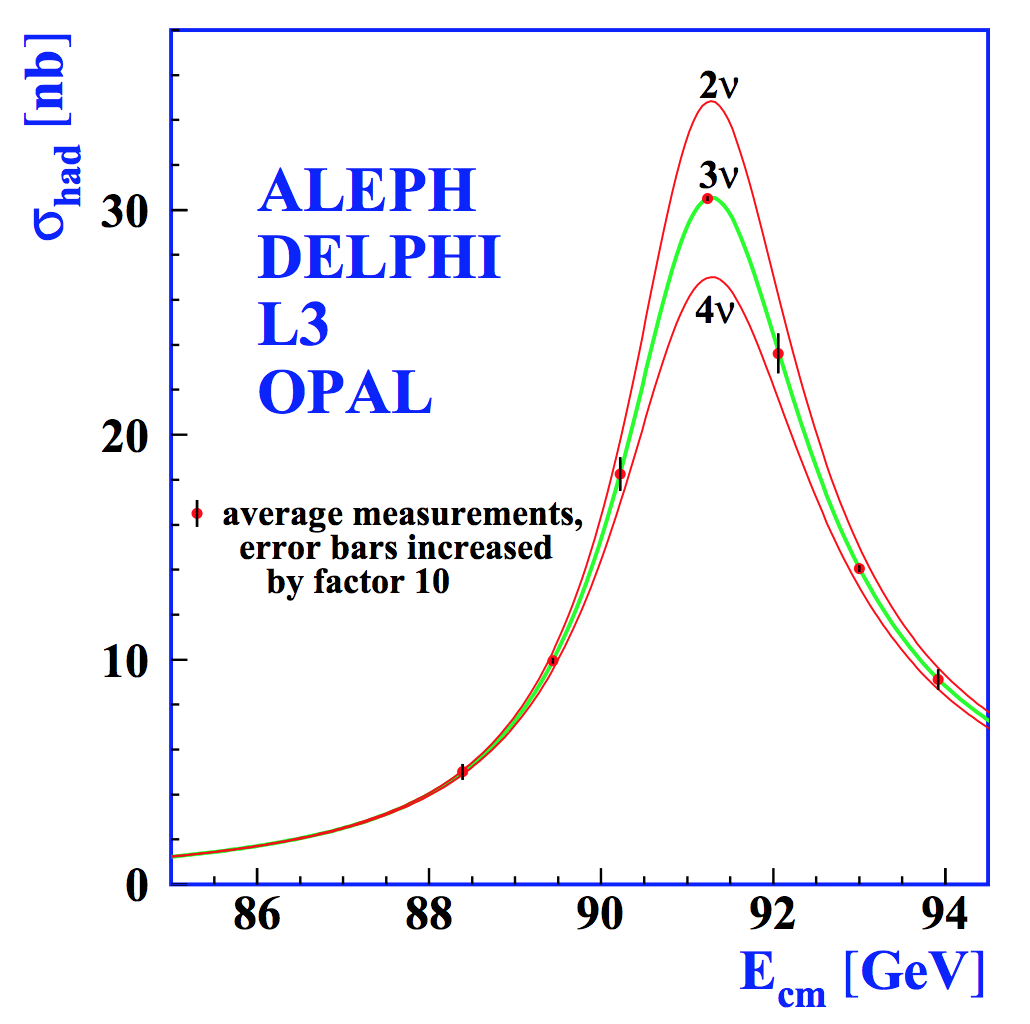
\includegraphics[width=0.5\linewidth]{ALEPH_NumNu.png} 
\caption[The number of neutrinos coupling to the Z from ALEPH]{The number of active neutrinos with a coupling to the Z boson as measured by ALEPH, DELPHI, L3, and OPAL. The data from the four experiments strongly favors only three neutrinos coupling to the Z boson. Image taken from \cite{ALEPH-3Nu}.}
\label{fig:ALEPH}
\end{figure}

\section{History of Cosmic Rays}
\label{sec:cosmic_rays}
In the early years of the 20th century, scientists began investigating previously-unknown ionizing radiation in the atmosphere.
Scientists using electroscopes, early instruments designed to measure electric charge and radiation, discovered low levels of radiation in the air.
This new radiation was observed to be reduced when the electroscope was shielded by metal free of radioactivity, indicating that the signal was not an artifact of the detector itself and was, instead, coming from an external source.

Following just a few decades after the discovery of radioactivity by Becquerel, many scientists believed that the electroscope was detecting radiation from the Earth itself.
The rate would be expected to decrease with increasing altitude above sea level and, to increase with increasing depth in the sea.
Early measurements by Domenico Pacini in 1910 showed that the radiation rate decreased by 20\% at a depth of 3 meters underwater compared to the rate at the surface \cite{Pacini-CRSource}, implying an origin independent of the Earth's crust.
Measurements were performed with electroscopes by Victor Franz Hess in 1912 of the rate of ionizing radiation up to an altitude of 5 km \cite{Hoerandel-CRHistory}.

Hess showed that the observed rate decreased until an altitude of around 1 km, but at a slower rate than expected from theory.
Above 1400 meters, however, the rate of ionizing radiation increased again, rising substantially up to the maximum altitude reached at 5300 meters \cite{Compton-CRAltitude}.
Hess's work, later confirmed by Henri Millikin, showed definitively that there exists a source of radiation of extraterrestrial origin, earning him the Nobel Prize in Physics for 1936 \cite{NobelPrize:1936-Hess}.
This radiation was later dubbed "cosmic rays" by Millikan in reference to their extraterrestrial origin.

\begin{figure}[!h]
\centering
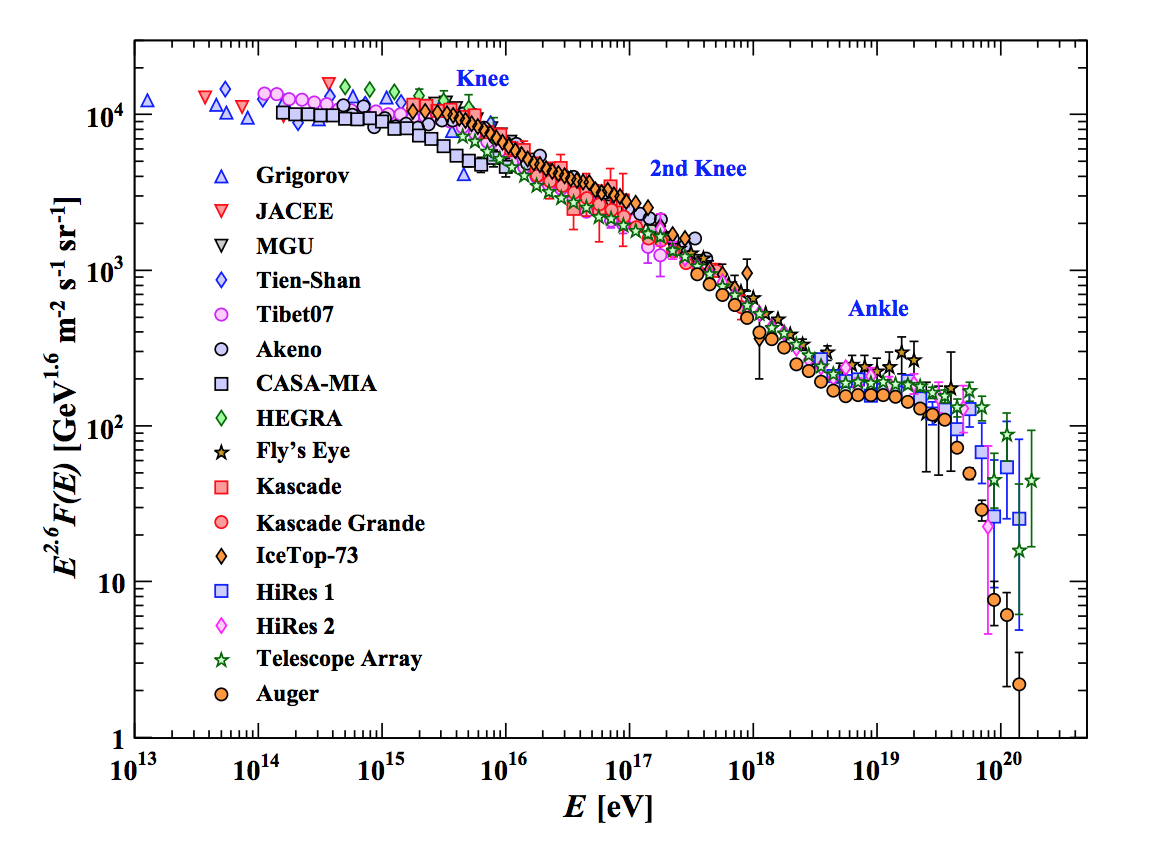
\includegraphics[width=0.9\linewidth]{CR_Spectrum_PDG15.png}
\caption[The cosmic ray spectrum as a function of energy]{The cosmic ray spectrum covers many orders of magnitude in energy and has been verified by many experiments to high precision. The various features are thought to be caused by multiple sources at different scales. Image taken from \cite{PDG-2015}}
\label{fig:CR_spectrum}
\end{figure}

The cosmic rays originally observed by Hess are now known to be primarily composed of protons and helium nuclei reaching the atmosphere from beyond the Earth.
Modern measurements have shown that the cosmic ray spectrum primarily consists of protons with a small contribution from helium and heavier elements \cite{PDG-2015}.
These ions are accelerated in astrophysical sources up to extremely high energies.
The cosmic ray spectrum extends over many orders of magnitude, with the highest energy observations reaching $\mathtt{10^{20}}$ electronvolts - far higher than any Earth-based accelerator.
The spectrum, shown in Figure~\ref{fig:CR_spectrum}, has multiple features that are believed to arise from different accelerator sources at different scales, each of which has been verified by multiple experiments.

Work on cosmic rays has lead to numerous discoveries.
In 1937, the first \emph{hadronic showers} were observed \cite{Blau-HadronicShowers}. 
Hadronic showers of particles created by interactions of cosmic rays were shown to produce large numbers of daughters \cite{Kolhoerster-CoincidenceDetectors, Hoerandel-CRHistory}.
These showers may result in the production of  $5\times10^6$ to over $10^9$ particles each \cite{CosmicRays-Extent}.
These showers begin with a cosmic ray primary particle, often a single proton accelerated to high energies, which interacts with particles of the Earth's atmosphere.
The interaction leads to the creation of various daughters, including muons, pions, kaons, and other hadrons and neutrinos.


\section{Atmospheric Neutrinos}
\label{sec:atmo_nus}
Air showers from cosmic rays provide a useful natural source of neutrinos in the GeV energy range and above that may be used for fundamental physics research.
The hadronic shower produces pions and kaons which decay to produce neutrinos 

\begin{equation}
\pi^+ \rightarrow \mu^+ \nu_\mu \rightarrow e^+ \nu_e \bar{\nu_\mu} \nu_\mu
\end{equation}

from the pions and from the kaons

\begin{equation}
K^+ \rightarrow \pi^+ \nu_\mu \rightarrow  e^+ \nu_e \bar{\nu_\mu} \nu_\mu \nu_\mu
\end{equation}

The resulting neutrino flux depends on a number of parameters, including the Earth's magnetic field and temperature profile, the cosmic ray flux, and the details of hadronic interactions in air showers \cite{Honda-2015}.
The calculation of the neutrino flux predictions requires significant, dedicated simulation work, producing fluxes as both a function of energy (Figure~\ref{fig:honda_en}) and direction (Figure~\ref{fig:honda_coszen}).

\begin{figure}[!h]
\centering
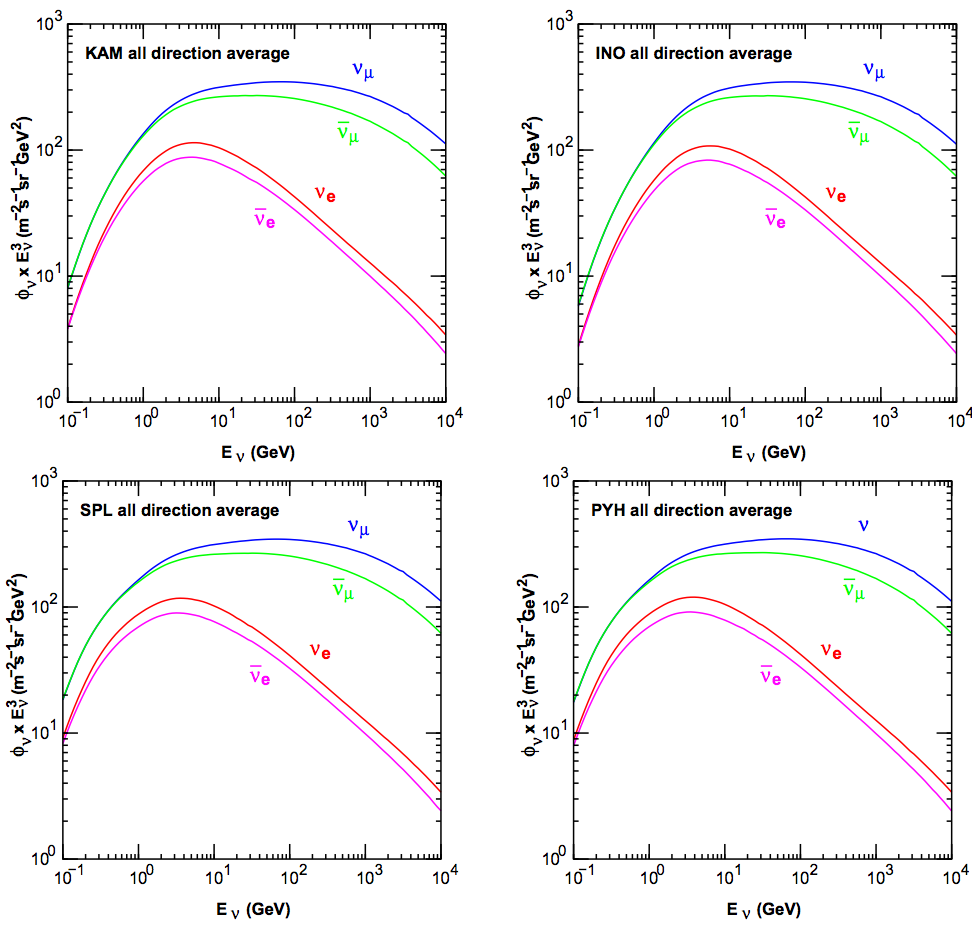
\includegraphics[width=0.6\linewidth]{honda15_en.png}
\caption[Expected neutrino flux as a function of energy]{The expected neutrino flux at Kamioka mine, Japan (Super-Kamiokande, top left), Ino Peak, India (India-based Neutrino Observator, top right), the South Pole (IceCube, bottom left), and Pyhasalmi mine, Finland (EMMA experiment, bottom right) as a function of energy. Note that the neutrino and anti-neutrino fluxes are characterized separately. The differences in the flux at each site is due to differences in the Earth's magnetic field and temperature profile. Figure taken from \cite{Honda-2015}.}
\label{fig:honda_en}
\end{figure}

\begin{figure}[!h]
\centering
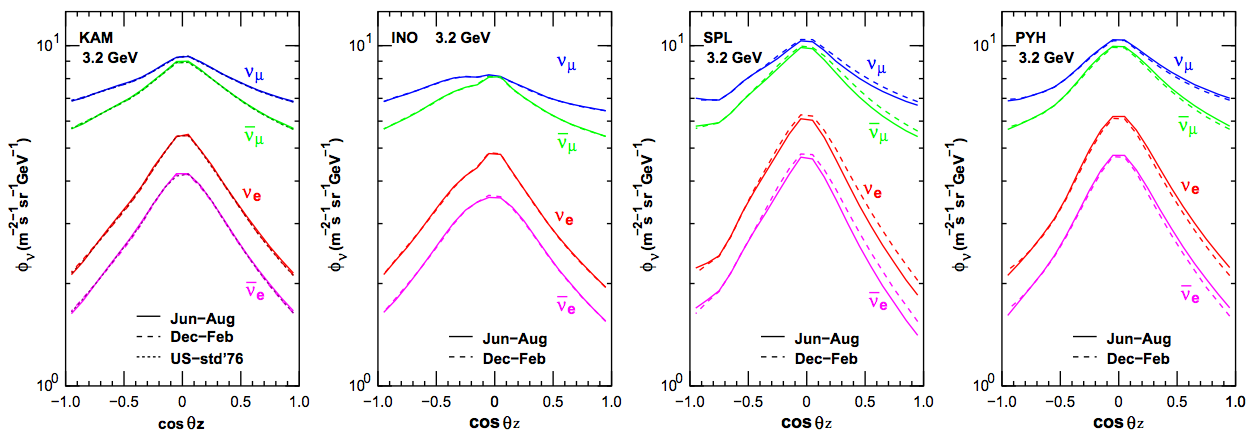
\includegraphics[width=\linewidth]{honda15_coszen.png}
\caption[Expected neutrino flux as a function of direction]{The expected flux of 3.2 GeV neutrinos at Kamioka mine, Japan; Ino Peak, India; the South Pole; and Pyhasalmi mine, Finland as a function of the cosine of the zenith angle. A value of $\cos \theta_Z=-1$ indicates neutrinos passing through the entire Earth and entering the detector from below while a value of $\cos \theta_Z=+1$ indicates neutrinos coming from the atmosphere directly above the detector. The differences in the flux at each site are due to differences in the Earth's magnetic field and temperature profile. Figure taken from \cite{Honda-2015}.}
\label{fig:honda_coszen}
\end{figure}

\section{The Standard Model}
\label{sec:standard_model}

\begin{figure}
\centering
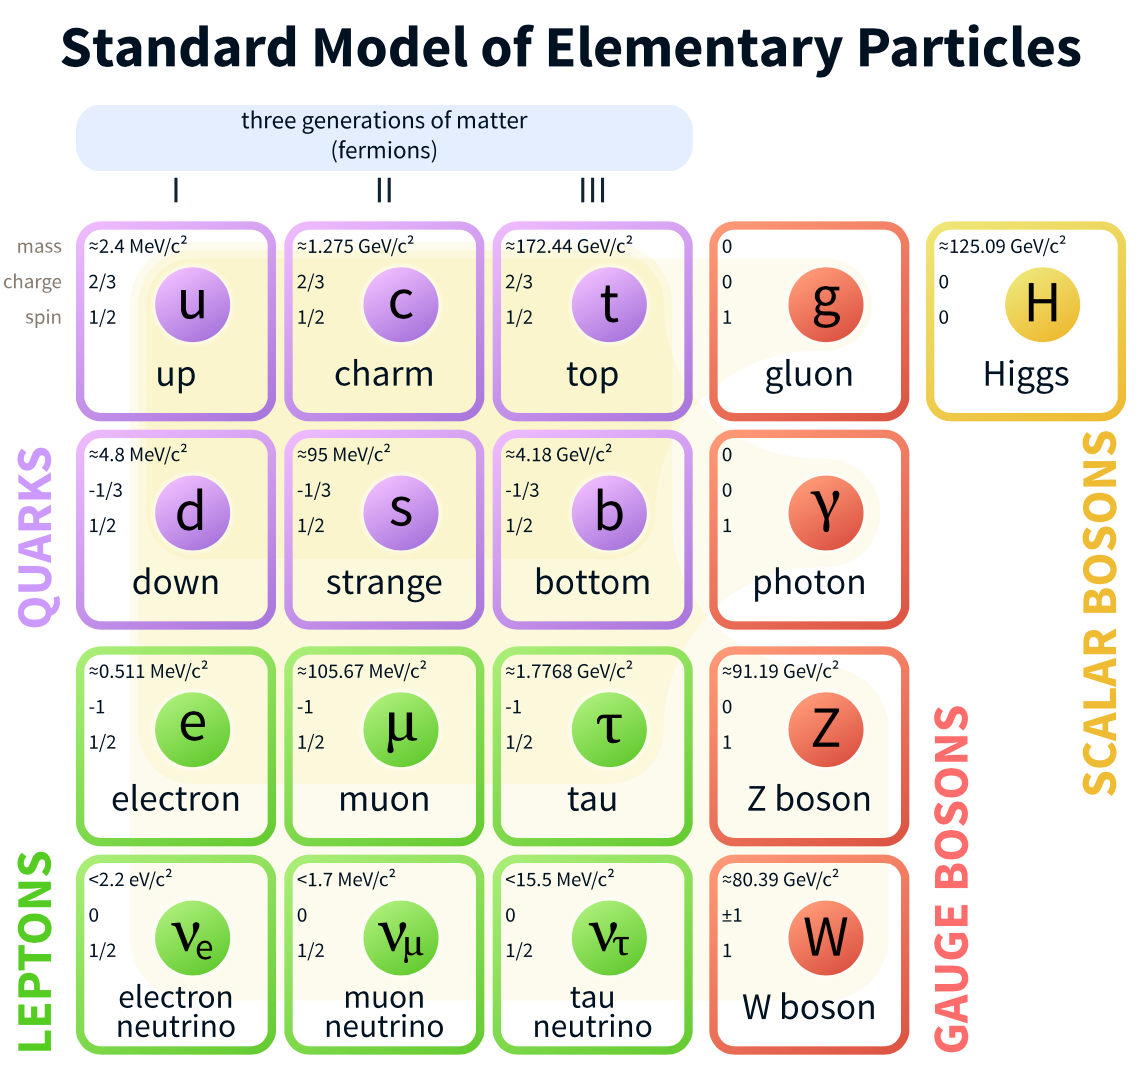
\includegraphics[width=0.7\linewidth]{Standard_Model_of_Elementary_Particles.png}
\caption[The Standard Model]{The Standard Model of particle physics is made up of charged and uncharged leptons, quarks, and the various bosons. Image taken from \cite{StandardModel-Image}.}
\label{fig:standard_model}
\end{figure}

Muons and neutrinos form just a small part of the Standard Model of particle physics.
The Standard Model, with fundamental particle types and properties shown in Figure~\ref{fig:standard_model}, consists of six quarks (up, down, strange, charm bottom, and top), three charged leptons (electron, muon, and tau), three uncharged leptons (electron neutrino, muon neutrino, and tau neutrino), and the five bosons related to interactions (photon, Z, W, gluon, and Higgs).
The Standard Model, developed over the last half century, elegantly encapulates the range of phenomena known to occur in particle physics and has been verified repeatedly over decades by many experiments, yielding precise checks on a wide range of parameters.

The three charged leptons and neutrinos form three "families" or "flavors". 
Each charged lepton is associated with a coupled neutrino which shares a lepton number that is conserved in interactions mediated by the W boson.
The electron, the lightest of the charged leptons at 511 keV \cite{PDG-2015}, is a key ingredient of the atoms that make up the world, is the only stable charged lepton.
The muon, with a mass of 105.7 MeV, is the middle of the three charged leptons, often appearing in particle interactions accompanied by the muon neutrino.
The muon has a relatively long livetime of 2.197 microseconds, far longer than many unstable hadrons.
The tau lepton is the heaviest of the leptons, and with a mass of 1.777 GeV, it is heavier than the proton and appears only in relatively high energy interactions.
The tau has an extremely short lifetime, at 290.6 femtoseconds, and a rich variety of decay products.
This extremely short lifetime and high mass make the tau difficult to produce and study.

For the purposes of this work, the most significant parts of the Standard model are the neutrinos, which will be defined to be signal events; the up and down quarks, which will make up the protons and neutrons upon which the neutrinos will interact; the W and Z bosons, which mediate the weak interactions via which the neutrinos may be observed; and the photon, which gives a method of observation of the interactions.

\subsection{Neutrino Interactions}
\label{subsec:interactions}
In the Standard Model, neutrinos are assumed to be massless, left-handed spin-1/2 leptons which interact solely via the weak force.
The neutrinos may also interact gravitationally, although gravity has no known representation in the Standard Model.
Neutrinos, therefore, are only visible via indirect effects, such as scattering or production of charged particles that may, in turn, give off their own visible signature.
An understanding of the methods by which neutrinos are detected therefore forms an important basis for the study of these elusive particles.
Two basic Feynman diagrams, shown in Figure~\ref{fig:nu_vertex}, represent the two major interaction vertices available for neutrinos.

\begin{figure}
\centering
\begin{tabular}{@{}ll@{}}
\feynmandiagram [vertical=w1 to w2] {
  nue1 -- [fermion, edge label=\(\nu\)] w1 -- [fermion, edge label=\(l\)] e1 ,
  w1 -- [boson, edge label = \(W^{+}\)] w2
}; 
 & \feynmandiagram [vertical=w1 to w2] {
  nue1 -- [fermion, edge label=\(\nu\)] w1 -- [fermion, edge label=\(\nu\)] nu2 ,
  w1 -- [boson, edge label = \(Z\)] w2
}; \\ 
\end{tabular}
\caption[Feynman diagrams for W, Z interactions of neutrinos]{Feynman diagrams showing the interaction vertex of the neutrino with the W and Z boson.}
\label{fig:nu_vertex}
\end{figure}

These two vertices describe the interactions relevent for the work presented in this thesis.
During \emph{charged current} (\emph{CC}) interactions, a $\mathtt{W^{\pm}}$ boson is exchanged between a neutrino and target particle(s), in the process converting the uncharged neutrino to the corresponding charged lepton.
The \emph{neutral current} (\emph{NC}) interactions are those in which the uncharged Z boson is exchanged with the target and the neutrino.
Although the neutrino can change energy and momentum, it does not get converted to a charged lepton.

Detectors used to study particle properties rely on electromagnetic interactions and photons in order to detect particles.
Because the neutrino itself does not interact via the electromagnetic force, charged leptons and hadrons must be used to indirectly study the properties of the incident neutrinos.
Outgoing charged leptons in charged current interactions may be detected, although the direction will not necessarily correspond to that of the incident neutrino. 
The average angle between the incident neutrino and outgoing lepton may be approximated following Equation~\ref{eqn:kinematic_angle},

\begin{equation}
\left<\bar{\theta}_{\nu l}\right> \approx \frac{\mathtt{1.5^o}}{\sqrt{E_\nu \left[TeV\right]}} .
\label{eqn:kinematic_angle}
\end{equation}

There exist three further classifications of neutral current and charged current neutrino interactions in the energy range used in this work: the quasi-elastic, resonant, and deep inelastic interactions \cite{Formaggio-Xsec}.
A fourth type, coherent neutrino scattering, may also occur, although the energies involved are too low to impact this work.
The three types of interactions are contribute to the total cross section with peaks at different energies, as shown in Figure~\ref{fig:xsec}.

\begin{figure}[h]
\centering
\begin{tabular}[b]{c}
  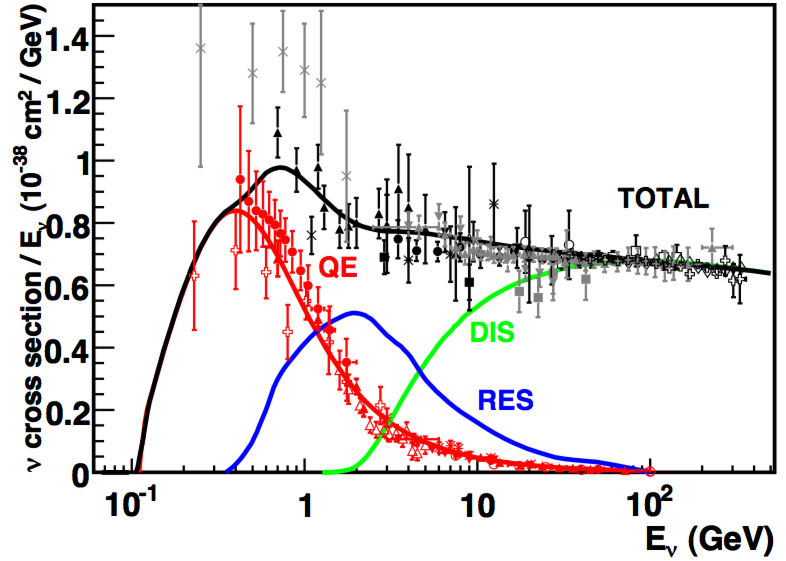
\includegraphics[width=0.45\linewidth]{nu_xsec_formaggio.png} \\
  \small (\textbf{\color{ctcolormain}a}) $\nu$ Interaction cross sections
\end{tabular} \hspace{2pt}
\begin{tabular}[b]{c}
  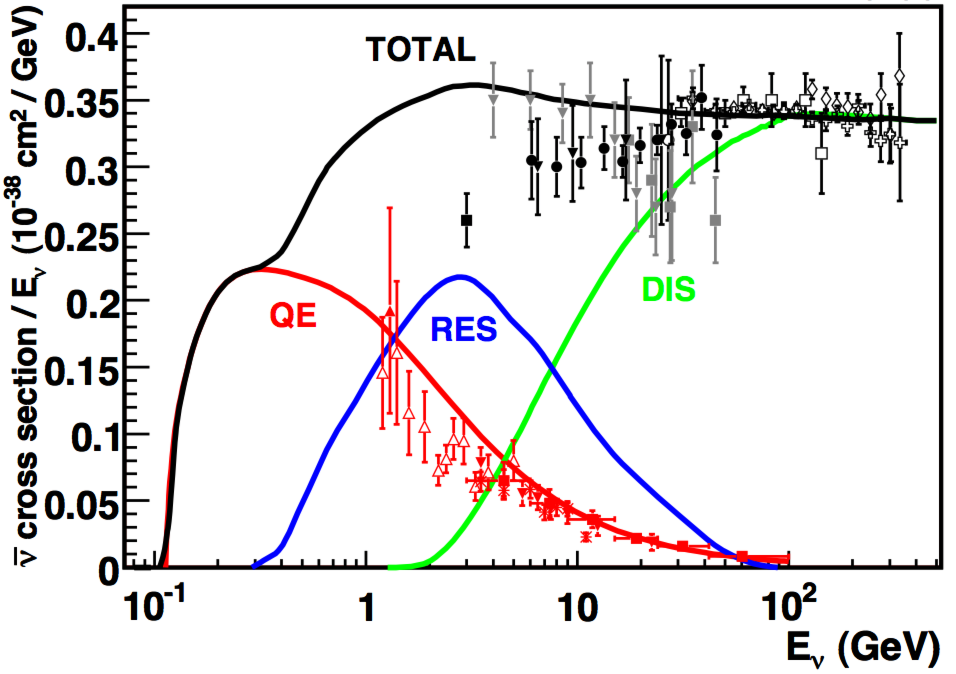
\includegraphics[width=0.45\linewidth]{nubar_xsec_formaggio.png} \\
  \small (\textbf{\color{ctcolormain}b}) $\bar{\nu}$ Interaction cross sections
\end{tabular}
\caption[QE, RES, and DIS cross sections for neutrinos]{The relative contributions to the cross section for $\nu$ (left) and $\bar{\nu}$ (right). The QE events dominate below 1 GeV while the DIS events dominate above 10 GeV. Note the different scales for the neutrino and antineutrinos. Images taken from \cite{Formaggio-Xsec}.}
\label{fig:xsec}
\end{figure}

\subsubsection{Quasi-Elastic and Resonant Interactions}
At low energies of approximately 100 MeV to around 2 GeV, the neutrinos predominantly interact via \emph{quasi-elastic scattering} (\emph{QE}) interactions.
In the QE interaction, the neutrino scatters off an entire nucleon instead of the individual quarks.
In a charged current QE neutrino (anti-neutrino) interaction, the target neutron (proton) is converted to a proton (neutron) while the neutrino is converted to a charged lepton.

The cross section for QE interactions depends on various nuclear form factors that must be fit to experimental data.
Many of these form factors may be fit to electron scattering data, leaving only the axial vector nuclear form factors to be measured in the neutrino sector \cite{Formaggio-Xsec}.
This form factor is normally assumed to have the dipole form 

\begin{equation}
F_A\left(Q^2\right) = \frac{g_A}{\left(1+\frac{Q^2}{M_A^2}\right)^2}
\label{eq:axial_mass_eq}
\end{equation}

where $\mathtt{g_A}$ is a constant fit to experimental data, $\mathtt{Q^2}$ is the 4-momentum transferred in the interaction, and $\mathtt{M_A}$ is the "axial mass".
This last term is fit to experimental data with a value of $\mathtt{M_A = 0.999 \pm 0.011}$ GeV \cite{Formaggio-Xsec}.

\emph{Resonant scattering} interactions (\emph{RES}), which result in the excitation of a nucleon followed by decay via emission of (typically) pions, occur for neutrinos of slightly higher energies of around 500 MeV to 10 GeV.
Resonant interactions are modeled in a similar way as the quasi-elastic interactions, with an associated axial mass term used to describe nuclear uncertainties.

\subsubsection{Deep Inelastic Interactions}
\begin{figure}
\centering
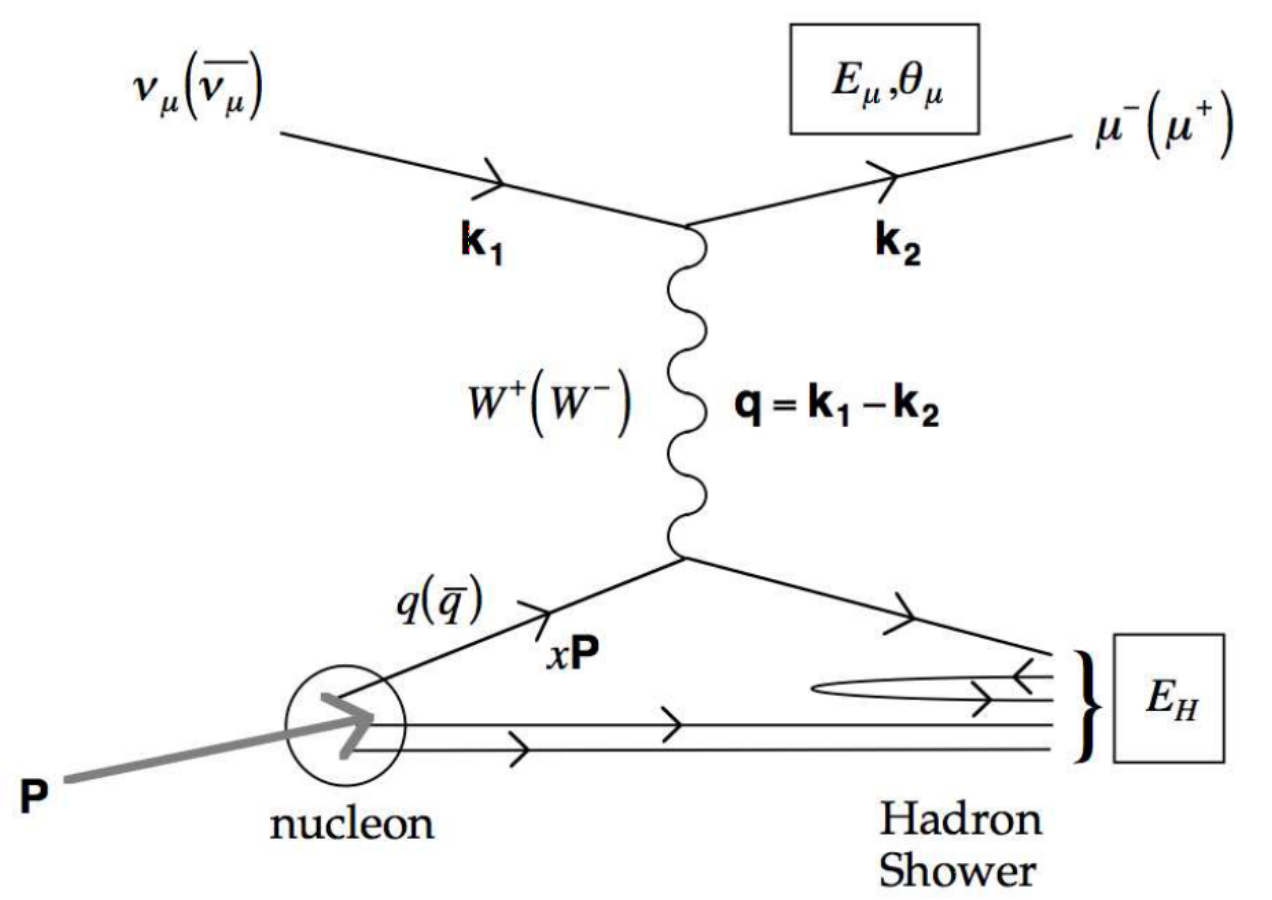
\includegraphics[width=0.5\textwidth]{dis_feynman.png}
\caption[A Feynman diagram of a charged current DIS neutrino interaction]{A Feynman diagram showing an example of a charged current neutrino DIS interaction. An incident muon neutrino interacts with a quark inside of a proton. The result is a hadronic shower as well as a charged muon. Diagram taken from \cite{Formaggio-Xsec}}
\label{fig:dis_feynman}
\end{figure}

Above a few GeV, the neutrino cross section rises approximately linearly with energy and is dominated by \emph{deep inelastic scattering} (\emph{DIS}) interactions.
An example of a DIS interaction is shown in Figure~\ref{fig:dis_feynman}.
In DIS events, the exchange of the Z or W boson probes the internal structure of the nucleons, leading to a scattering off of the individual nucleons.
This results in disruption of the nucleon and the larger nucleus and a collection of daughter particles forming a \emph{hadronic shower}.

As seen in Figure~\ref{fig:xsec}, the DIS process dominates the neutrino cross section above 10 GeV and form the only significant interaction above 100 GeV \cite{Formaggio-Xsec}. 

\section{Methods of Detection}
\label{sec:detection_methods}
Neutrinos may be detected through the QE, RES, and DIS interaction channels.
The interaction of neutrinos at the GeV energy ranges relevent for this thesis lead to the emission of hadrons in a hadronic shower.
The QE interactions at low energies convert neutrons into protons (neutrino) or protons into neutrons (antineutrino) and emitting a charged lepton.
RES interactions excite a nucleon, leading to a deexcitation and emission of particles that can be detected.
DIS interactions produce larger hadronic showers containing many charged particles.

In addition to the hadronic shower, charged current interactions result in an outgoing charged lepton, the result of which depends on the flavor of the incident neutrino.
Outgoing electrons quickly scatter in interactions with the surrounding media, ionizing atoms and producing a secondary \emph{electromagnetic shower} of particles.
Muons, on the other hand, travel longer distances before scattering or decaying in the medium, leading to an extended track.

\begin{table}[]
\centering
\begin{tabular}{@{}lll@{}}
\toprule
Decay                                     & Branching Ratio     & Background   \\ \midrule
$\tau \rightarrow e^- \nu_e \nu_\tau$     & 17.83 $\pm$ 0.04 \% & $\nu_e$ CC   \\
$\tau \rightarrow \mu^- \nu_\mu \nu_\tau$ & 17.41 $\pm$ 0.04 \% & $\nu_\mu$ CC \\
$\tau \rightarrow$ hadrons                & Otherwise           & $\nu$ NC     \\ \bottomrule
\end{tabular}
\caption[Branching ratios for the tau lepton decay]{The branching ratios for the decay of tau leptons. Two-thirds of the time, the tau lepton decays hadronically.}
\label{tab:tau_decays}
\end{table}

The signature of a tau neutrino charged current interaction varies depending on the specific decay channels, shown in Table~\ref{tab:tau_decays}.
Because the tau lepton has a very short lifetime, outgoing taus from charged current tau neutrino interactions tend to decay immediately.

Each of the three decay modes mimic interactions of the electron and muon neutrinos.
The decay to an electron or hadrons produces electromagnetic or hadronic showers respectively.
The secondary electromagnetic or hadronic cascade is theoretically distinguishable from the primary hadronic cascade produced by a tau neutrino charged current interaction, although the distance traveled by the tau lepton at the energies used in atmospheric oscillation measurements, around 10 GeV, is on the order of millimeters.

In each case, the charged particles deposit energy into the interaction medium through a series of stochastic and continuous emissions.
It is through the detection of these stochastic and continuous losses that daughter particles may be identified in the study of neutrinos.

\subsection{Stochastic Emission Mechanisms}
A total of five major stochastic emission mechanisms are important for the energy losses in neutrino experiments \cite{Dima-MMC}:
ionization, bremmstrahlung, pair production, 

The decay of the particle splits the energy of the parent into multiple, lower energy daughters.
Decays of daughter leptons can often by important in the identification of the neutrino flavor, particularly for tau neutrino candidates occuring above 10 TeV when the primary and secondary hadronic interactions become well-separated.

Ionization losses occur when the charged lepton interacts with electrons in the medium, transferring enough energy to librerate the electrons from bound states.
At energies below 1 TeV, these losses are the most significant form of energy loss for charged particles, producing a significant source of additional electrons.
Ionization losses occur roughly independently of the energy of the charged lepton.

Above energies of a few hundred GeV, radiative processes dominate the energy losses for muons in matter \cite{PDG-2015}.
Bremmstrahlung, photon emission from charged particles accelerating in a magnetic field, pair production, in which a particle and antiparticle (typically electron and positron) are created, and hadronic interactions of photons all dominate the energy losses of muons above 1 TeV.

There exists a minimum in the energy loss rates.
Particles emitting near this minimum rate are known as \emph{minimum-ionizing} particles \cite{PDG-2015}.

\begin{figure}
\centering
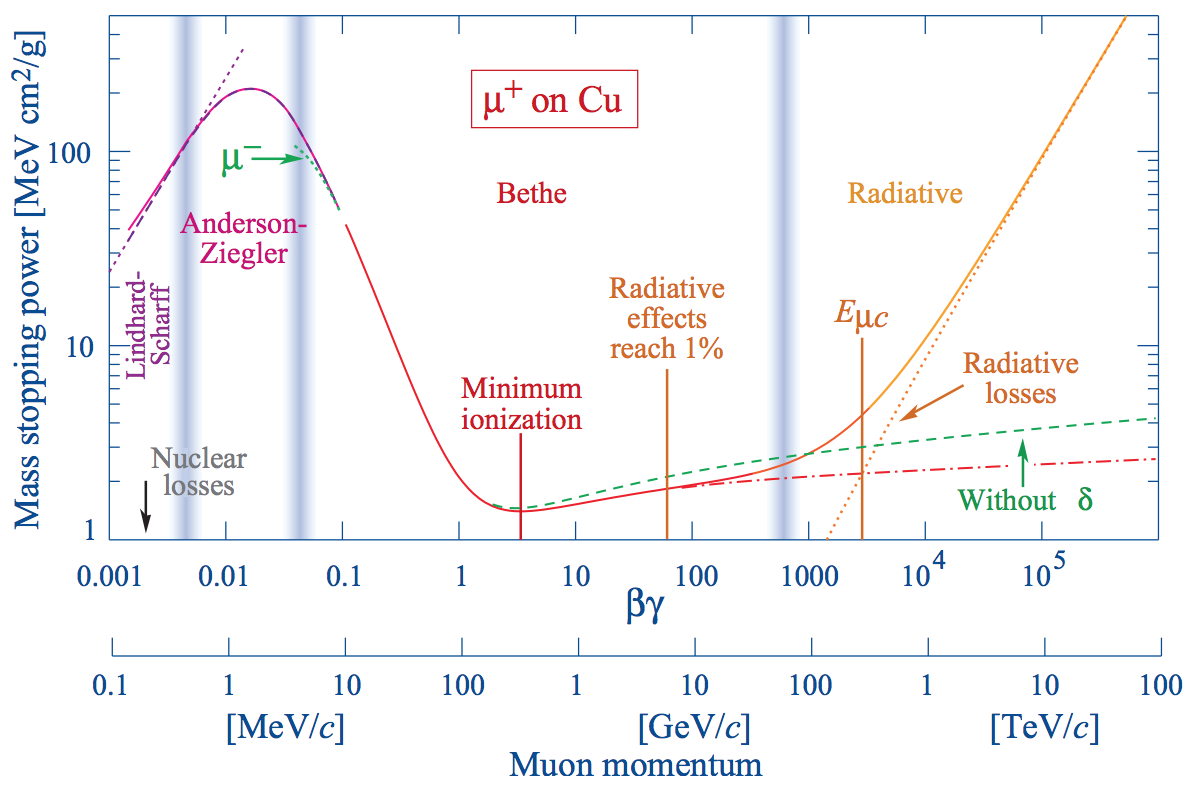
\includegraphics[width=0.8\linewidth]{bethe_bloche-PDG15.png}
\caption[Energy losses of a muon in matter]{An example of the energy loss ($\mathtt{\frac{-dE}{dX}}$) calculated for muons incident on copper. The radiative losses due to bremsstrahlung, pair production, and photonuclear interactions are dominant above 1 TeV. Note the labeled minimum of the curve showing the energy losses of a minimum ionizing particle. Image taken from \cite{PDG-2015}.}
\label{fig:discrete_emissions}
\end{figure}

Stochastic emissions result in additional particles in the detector, leading to improved light yield.
In addition, some detectors use photosensitive emulsions  \cite{Description-OPERA, DONUT-2001}, scintillators \cite{Description-MINOS, Description-NOvA, Description-MINERvA, Description-T2K}, or time projection chambers \cite{Description-ICARUS2} in order to track ionization losses.
These emulsions yield precise characterization of particle decays, allowing experimentalists to uniquely determine the flavor state of the interacting neutrino.

\subsection{Cherenkov Emission}
When a charged particle passes through a dielectric medium with a speed larger than the local phase velocity of light, it will emit \emph{Cherenkov radiation}\cite{Cherenkov-Radiation-Confirmation}.
The effect, first reported by Pavel Cherenkov in 1934 \cite{Cherenkov-Radiation-Observation} remained unexplained theoretically until work done by Ilya Frank and Igor Tamm in 1937 \cite{Frank-Tamm}.

For a dielectric medium, the electric field of charged particle will polarize atoms, inducing a small dipole moment in atoms in the medium \cite{Griffiths-EM}.
The resulting disturbance of the medium propagates with the phase velocity of light, given by the speed of light, \textit{c}, and the index of refraction as a function of the frequency of light, \textit{n(\omega)}.
If the charged particle is traveling faster than the local phase velocity, the electromagnetic disturbance propagates with constructive interference, resulting in a planar wavefront of emission known as \emph{Cherenkov emission}.
The angle of the wavefront relative to the propagation direction is given by the ratio of the distance traveled by the particle and photons in a given time,

\begin{equation}
cos(\theta_C) = \frac{\frac{c}{n(\omega)} t}{v t} = \frac{c}{n(\omega) v} 
\end{equation} 

where $\theta_C$ is the \emph{Cherenkov angle}, $v$ is the speed of the particle.
The energy threshold for Cherenkov emission is set by a combination of the particle mass and the local phase velocity for light, $\frac{c}{n}$.
Using the relativitistic kinetic energy \cite{Tavernier-Particles},

\begin{equation}
\begin{tabular{c}
E_{C} \geq \frac{mc^2}{\sqrt{1-\left(\frac{c/n}{c}\right)^2}} \\ \\

E_{C} \geq mc^2\sqrt{\frac{n^2}{n^2-1}}.
\end{equation}

For ice with a index of fraction of 1.32 at 400 nanometers \cite{ChinesePhysC-2014}, this works out to a minimum energy of 270 keV for electrons and 56.2 MeV for muons.
The number of photons emitted increases with photon energy, with approximately 50\% more photons produced in blue visible light than in red\cite{Tavernier-Particles}
The full emission spectrum, first worked out by Ilya Frank and Igor Tamm in 1937 \cite{Frank-Tamm}, depends on a number of parameters, including the energy and charge of the emitting particle as well as the properties of the medium.
In the case of a particle traveling a distance $L$ much larger than the photon frequency of interest, $\lambda$, the number of emitted photons may be approximated by

\begin{equation}
\frac{dN}{d\lambda}=\frac{2\pi \alpha}{\lambda^2}Lsin^2\theta_C \;\;\; L >> \lambda
\end{equation}

where $\alpha$ is the fine structure constant.

Cherenkov emission is not limited to a single charged lepton. 
All charged particles emit Cherenkov radiation, including any hadrons and charged daughter particles.
While the total amount of energy lost via Cherenkov emission is small relative to losses due to stochastic processes, this emission type is both continous and results directly in photons which may be observed by photodetectors.
This technique is used by multiple experiments, including SNO \cite{Description-SNO}, Super-Kamiokande \cite{Description-SuperK}, ANTARES \cite{Description-ANTARES}, and IceCube \cite{Description-IceCube}.

